\documentclass[11pt,a4paper]{article}
\usepackage[margin=0.85in]{geometry}
\usepackage{fontspec,unicode-math,booktabs,graphicx,hyperref}
\setmainfont{STIXGeneral}\setmathfont{STIX Two Math}
\title{Complete comparisons using the available authored texts}
\author{Human Compression project}\date{}
\begin{document}\maketitle
Two missing PDFs need not prevent comparison of the available manuscripts.
For Buekenhout and Cara's \emph{Some properties of inductively minimal
geometries} (1998, N001), and Bonheure, Buekenhout and Leemans's
\emph{On the Petrials of thin rank 3 geometries} (2001, L108), the complete
authored renderings are available. Both contain all seven printed pages,
including references and final author matter. The saved and newly retrieved
bodies agree. An independent review checked the complete boundaries and
all twenty counts. It removed one website trailer after N001's final address.

The primary comparison counts NFC characters without whitespace in every
complete authored document. Running headers and page numbers remain
included on both sides. N001 and L108 use their literal authored renderings;
all other originals and all replacement papers use untrimmed PDF text.
This is a comparison of the available text representations. Missing figure
information and unverified formula glyphs are not reconstructed.
The previous PDF-only comparisons remain unchanged historical records.

The declared principal-result contracts and their qualifications are exactly
those of the accepted B and C editions. No additional result or conjecture
is proved by measuring them. Each topic pays for its own entire common
theory once. Individual factors assume that theory has been acquired;
Topic C also assumes both complete required programs have been acquired.
There is no discount between topics. Expanded external proofs and complete
graphic costs remain unknown. These lengths are not minimum proof lengths.

\newpage
\section*{Topic B: Forest coordinates and primitive geometries}
\begin{center}\begin{tabular}{lrrr}\toprule Source/application & Source cost & Application cost & Conditional factor\\\midrule
N001/B1 & 14519 & 7371 & 1.970\\
N003/B2 & 17780 & 14170 & 1.255\\
N008/B3 & 18009 & 11132 & 1.618\\
L030/B4 & 22704 & 12286 & 1.848\\
\bottomrule\end{tabular}\end{center}
The entire common paper costs 14,124 characters; the four applications cost 44,959. Thus
\[R_B=\frac{73012}{14124+44959}=\frac{73012}{59083}=1.235753.\]
These proofs require no finite mathematical program. All four sources remain in the numerator and all four applications remain in the denominator.
\begin{center}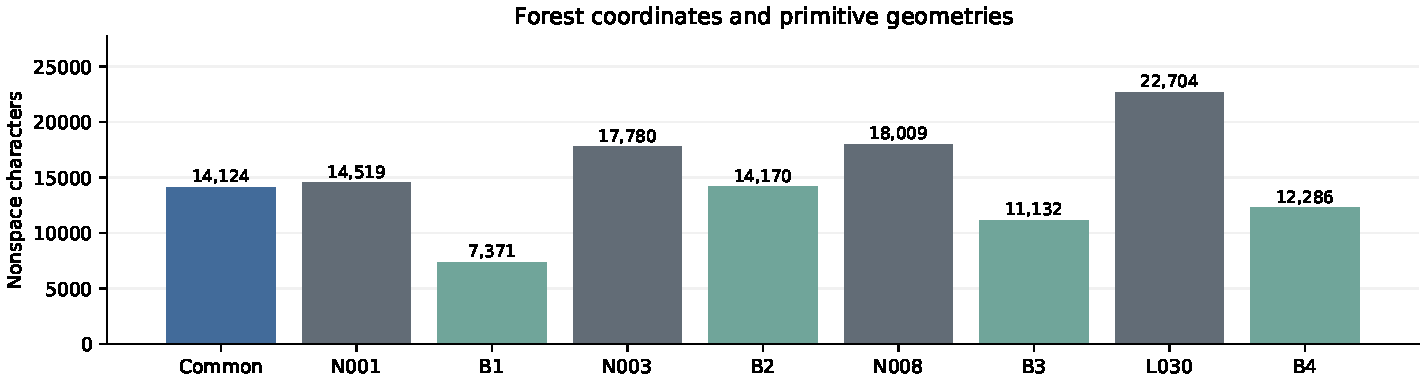
\includegraphics[width=\textwidth]{B-costs.pdf}\end{center}
The graph shows acquisition of the complete common paper, followed by each matched original and application in the established application order. It does not by itself establish a recurring sawtooth pattern.
\paragraph{Unit sensitivity.} All documents remain untrimmed in this table.\begin{center}\begin{tabular}{lr}\toprule Unit & Whole written factor\\\midrule
Whitespace words & 1.370\\
Alphanumeric units & 1.406\\
Nonspace characters & 1.236\\
Characters, collapsed spaces & 1.259\\
UTF-8 bytes, collapsed spaces & 1.184\\
\bottomrule\end{tabular}\end{center}
The machine-readable results retain both normalizations and all five units. Comparisons with selected or calibrated PDF text are labelled separately as mixed-boundary sensitivities; they are not the primary factors above. Literal rendered-source counts remain fixed in those variants.

\newpage
\section*{Topic C: Chamber operations and binary translations}
\begin{center}\begin{tabular}{lrrr}\toprule Source/application & Source cost & Application cost & Conditional factor\\\midrule
L088/C1 & 13166 & 11311 & 1.164\\
N013/C2 & 27361 & 15815 & 1.730\\
L108/C3 & 12849 & 10075 & 1.275\\
F014/C4 & 20577 & 6962 & 2.956\\
\bottomrule\end{tabular}\end{center}
The entire common paper costs 27,142 characters; the four applications cost 44,163. Thus
\[R_C=\frac{73953}{27142+44163}=\frac{73953}{71305}=1.037136.\]
The complete printed program appendix costs 8,803, giving 0.923166. Both whole raw programs cost 8,323 instead, giving 0.928731. These program representations are alternatives, never two simultaneous charges.
\begin{center}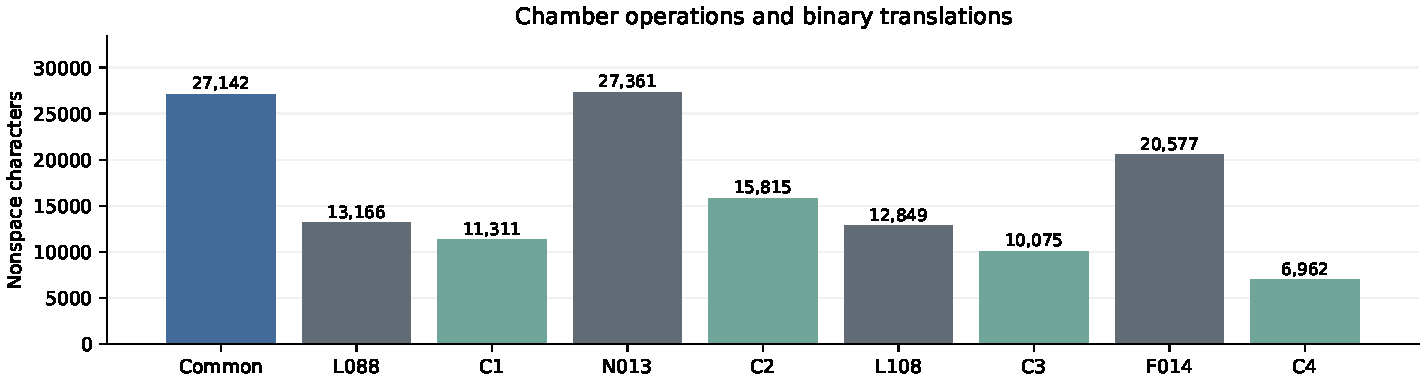
\includegraphics[width=\textwidth]{C-costs.pdf}\end{center}
The graph shows acquisition of the complete common paper, followed by each matched original and application in the established application order. It does not by itself establish a recurring sawtooth pattern.
\paragraph{Unit sensitivity.} All documents remain untrimmed in this table.\begin{center}\begin{tabular}{lr}\toprule Unit & Whole written factor\\\midrule
Whitespace words & 1.188\\
Alphanumeric units & 1.154\\
Nonspace characters & 1.037\\
Characters, collapsed spaces & 1.063\\
UTF-8 bytes, collapsed spaces & 1.005\\
\bottomrule\end{tabular}\end{center}
The machine-readable results retain both normalizations and all five units. Comparisons with selected or calibrated PDF text are labelled separately as mixed-boundary sensitivities; they are not the primary factors above. Literal rendered-source counts remain fixed in those variants.

\end{document}
